\documentclass[a4paper]{article}
\usepackage{lipsum}
\usepackage{url}
\usepackage{graphicx}
\usepackage{indentfirst}
\usepackage{xcolor}
\usepackage[margin=2cm]{geometry}
\usepackage{lmodern}
\usepackage{enumitem}
\renewcommand{\familydefault}{\sfdefault}
\graphicspath{ {images/} }

%Custom Commands
\newcommand{\Pokemon}{Pok\'{e}mon}

%NOTE: 2,000 Words / 4 Pages
%NOTE: Make the Work Plan codes more detailed

%TODO: Get a better font and layout :P
%TODO: Think of a better title?
%TODO: Make sure work plan description titles follow a sensible structure and match
%TODO: Check whether the Rules reference is relevant of if I can get a better one
%TODO: Look into font size

\begin{document}

%Title Information
\title{
    Project Proposal
    \\ \large{G54IRP/COMP4027}
    \\ \large{Project Title: AI for General Video Game Playing}\vspace{-3ex}}
\author{4262648 Benjamin Charlton (psybc3)}
\date{\vspace{-2ex}22\textsuperscript{nd} October 2018}
\maketitle

\section{Background and Motivation}
\subsection{AI Game Playing}
Game playing has often been used in Artificial Intelligence (AI) research to help push the field forward, developing new techniques to tackle harder and harder problems.
Many of these AI techniques developed have since been applied to further applications proving that this field of study is not just producing novel solutions.
\par
Game Playing is a good playground to test AI techniques as games have many features that are helpful to testing AIs.
Some of the following reasons show why games make good AI problems:
\begin{itemize}[noitemsep,nolistsep,leftmargin=*]
  \item Clear win states leading to easy objective evaluation
  \item Limited actions creating fewer output options
  \item Well defined documentation allowing for precise and simple simulations
  \item Testing against different game types as defined in Game theory, such as imperfect information, stochastic outcomes, asymmetric gameplay etc.
  \item Ability to test and rank AIs against human players
\end{itemize}
\par
The history of AI game playing begins near the start of artificial intelligence as a field, in the 1950s.
Strachey created a draughts player for one of the first general computing machines (Manchester Ferranti Mark I) which by  1952 could ``play a complete game of draughts at a reasonable speed''\cite{BreifHistoryComputing}.
Prinz wrote a simplified chess player for the Manchester Machine as well which could solve the mate-in-two, which if there was a checkmate solution in 2 turns it could find it\cite{BreifHistoryComputing}.
\par
Currently most simple board games have been solved with AI techniques.
In 1997 IBM managed to beat the reigning world champion, Garry Kasparov, using Deep Blue.
Deep Blue used a combination of alpha-beta search trees with specialised hardware to generate the possible moves\cite{deepBlue}.
Google DeepMind recently took a long standing goal of AI game playing by beating a GO champion with AlphaGo\cite{AlphaGo}.
This done using a Monte Carlo Tree Search with the moves it chooses from being learnt from training a deep neural network that has been trained on human and computer play.
AlphaGo was then extended by Google DeepMind to create AlphaGoZero which didn't train with human data only self play\cite{alphaGoZero}.
\par
\begin{itemize}
    \item History of Video Game AI playing
    \begin{itemize}
        \item In Game AI
        \item Game Playing
    \end{itemize}
    \item General AIs
    \item Motivation
\end{itemize}

% @MISC{openAI,
%     author = {T.C. Sottek},
%     title = {The world’s best Dota 2 players just got destroyed by a killer AI from Elon Musk’s startup},
%     month = aug,
%     year = {2017},
%     howpublished = {\url{https://www.theverge.com/2017/8/11/16137388/dota-2-dendi-open-ai-elon-musk}}
% }
%
% Initially this has been seen with traditional board games like Chess[1] and Go[6]. During The International 2017 for DotA 2 this all changed as the worlds of AI and eSports came together in a 1v1 show match[8]. Elon Musk, backer of this initiative, said that this is ‘Vastly more complex than traditional board games like chess & Go’[8].Typically in these set ups their is no decisions to be made prior to the game itself, in fact to limit the DotA 2 AI they limited it to a preselected character to play with.

\section{Aims and Objectives}
This research project sets out to create and implement a General AI to play video games.
To test and evaluate this goal the solution developed will be tested against the GVGAI framework using the competition rules.\cite{GVGAI2014}
The project will produce an AI to play in the GVGAI framework as well as a research paper describing the performance of the AI created.
The objectives of this project are as follows:
\begin{description}
    \setlength{\parskip}{0pt}
    \item [Background Research]
    Perform research into the current state of AI game playing, general AIs, and current well performing solutions to the GVGAI competition.
    The result of this background study will be used to direct the rest of the project and determine a suitable method to tackle the problem with.

    \item [Design a General AI]
    Design an AI suitable to playing general video games as presented in the GVGAI framework.
    The design and approach will be heavily influenced by the research performed earlier in the project, taking account of other previous methods both in and out of the general game playing field as well as how the problem is presented in the framework.

    \item [Develop a General AI]
    Implement and develop the design created to tackle the problem.
    This will be the primary output of the project.
    Due to the heavy reliance on the background research it isn't clear what this stage will involve.

    \item [Evaluation and Analysis of Solution]
    Compare and analyse the performance of the solution against the other entries to the GVGAI competition and potentially against human players.
    If the solution performs well there may be the ability to test them in unseen environments, such as Video Games that aren't shown in the training sets.
\end{description}

\section{Work Plan}
To help outline the project scope and schedule, a gantt chart (found in the appendix) has been created.
High level descriptions of all of the subtasks have been written out as follows.
Some parts of the work plan (specifically development) are currently very vague as the initial research needs to happen to acquire the knowledge and insight of how to proceed.
\par
Updates to the work plan will happen to break down these tasks in to more concrete steps with accurate timeframes once the direction of the project is better known.
Additional updates will also come to better reflect how long certain parts of the project will take if adjustments need to be made due to events such as increase of scope or additional commitments.

%Explanations of all of the Points on the work plan
\begin{description}
\setlength{\itemsep}{0pt}
\setlength{\parskip}{0pt}
\item [\large{Documentation}]
\item [D1--Project Proposal Draft]
Write the project proposal draft for approval and feedback from supervisor, due 12\textsuperscript{th} October.
\item [D2--Project Proposal Finalise]
Any revisions to the project proposal that need to be made after supervisor feedback, due 22\textsuperscript{rd} October.
\item [D3--Preliminary Ethics Checklist]
Fill out and submit the preliminary ethics checklist, no further ethical checks should be required so no further time is scheduled.
\item [D4--Interim Report Outline Sections]
Create a basic outline of how the interim report will look with respect to the sections included and their content
\item [D5--Interim Report Related Work]
Write the related work section of the interim report, discussing previous research in General AI and game playing.
This will happen alongside the research steps that correspond to this task.
\item [D6--Interim Report Draft]
Create a draft of the interim report with all sections roughly finished.
\item [D7--Interim Report Finalise]
Add the finishing touches to the interim report summarising the work so far, due 7\textsuperscript{th} December.
\item [D8--Research Paper Structure Sections]
Outline the sections of the research paper and what content will be in each section.
\item [D9--Research Paper Abstract]
Write the abstract for the research paper.
\item [D10--Research Paper Draft]
Create a draft of the entire research paper with all sections roughly finished.
\item [D11--Research Paper Video Demo]
Create the demo video that needs to be submitted alongside the research paper.
\item [D12--Research Paper Finalise]
Final touches to the research paper, due 12\textsuperscript{th} April.
\end{description}

\begin{description}
\setlength{\itemsep}{0pt}
\setlength{\parskip}{0pt}
\item [\large{Research}]
\item [R1--Background Research]
Background research into the problem and history of the field for the Background section of the project proposal, as well as research into the module structure to help plan out the project.
\item [R2--GVGAI Basic Research]
Basic research into the structure and aims of the GVGAI competition.
\item [R3--GVGAI Framework Review]
Look into the structure and features of the GVGAI framework, happening alongside implementing a random agent.
This will help with development of this agent and inform the complexity of the problem for future planning.
\item [R4--GVGAI Papers for Related Works]
Background research into previous attempts at the GVGAI competition, looking into successful methods and analysis of the problem to better formulate a new approach to the problem.
\item [R5--Other Related Works]
Background research into further related works to the problem, looking into AI game playing and general AI problem solving.
\item [R6--Research for Solution]
Rough allocation of time to allow further research into a chosen method.
This will be broken into subtasks with better timeframes depending on the chosen method to tackle the problem.
\end{description}

\begin{description}
\setlength{\itemsep}{0pt}
\setlength{\parskip}{0pt}
\item [\large{Development}]
\item [S1--Install GVGAI Framework]
Install the components of the GVGAI framework.
\item [S2--Implement Random Agent]
Implement an agent that performs random actions, this won't score well but will show that the framework is working and will help with familiarity of the framework.
\item [S3--Run available previous agents]
If available, find and run some previous solutions to the GVGAI problem.
\item [S4--Develop Solution]
Rough allocation of time to allow development of the chosen method.
This will be broken into subtasks with better timeframes depending on the chosen method to tackle the problem.
Currently vague as the sub tasks involved in this step will depend on the method chosen to tackle the problem.
\end{description}

\begin{description}
\setlength{\itemsep}{0pt}
\setlength{\parskip}{0pt}
\item [\large{Presentation}]
\item [P1--Presentation General Outline]
Begin work on the presentation outlining the general content and flow.
\item [P3--Create Demo for Presentation]
Create a demo of the project to show how it performs.
\item [P3--Finalise Presentation]
Make final adjustments to the presentation and practice delivering it in its final form.
\item [P4--Present Presentation]
Present the presentation and demo during the demo day.
\end{description}

\begin{description}
\setlength{\itemsep}{0pt}
\setlength{\parskip}{0pt}
\item [\large{Miscellaneous}]
\item [M1--Create Git repository]
Create a Git repository on the School of Computer Science Git server to allow for management of the code and documentation.
\item [M2--Install LaTeX]
Install LaTeX and any other dependencies to allow production of documentation through out the project.
\item [M3--Create Meeting Minute Document]
Create a document to keep track of meetings with project supervisor.
This will be added to after every meeting but initial setup happens during this time.
\item [M4--Plan 2nd Stage of the Project]
Time set aside to plan out the 2nd stage of the project involving a the research and development of the solution.
This is mostly breaking down tasks R6 and S4 into precise subtasks.
\item [M5--Print and Collate Final Hand In]
Time to print and collate the final documentation required for the main hand.
This will involve properly packaging both digital and physical files.
\item [M6--SET/SEM Questionaries]
Module feedback to be completed. Student Evaluation of Teaching and Student Evaluation of Modules to comment upon supervisor teaching and the module as a whole respectively.
\end{description}

\begin{description}
\setlength{\itemsep}{0pt}
\setlength{\parskip}{0pt}
\item [\large{Other Commitments}]
\item [C1--Welcome Weeks]
First weeks of the academic year, time set aside to allow for settling in as well as running various welcome events.
\item [C2--Christmas Holiday]
Time off after Autumn term, Partially set aside to all for a break and time to relax.
\item [C3--Autumn Exams]
Potentially could have exams during the entire 2 weeks so is set aside to allow for revision and the exams themselves.
This can be updated to give a better reflection of when exams will be at a later date.
\item [C4--Easter Holiday]
Time off after Spring term, As no teaching is happening will give more time to concentrate on coursework and the presentation.
\end{description}

\section{Appendix}
%Bibliography
\bibliography{ProjectProposal}
\bibliographystyle{plain}

%Work Plan
\clearpage
\begin{center}
    \Large{Work Plan}\\
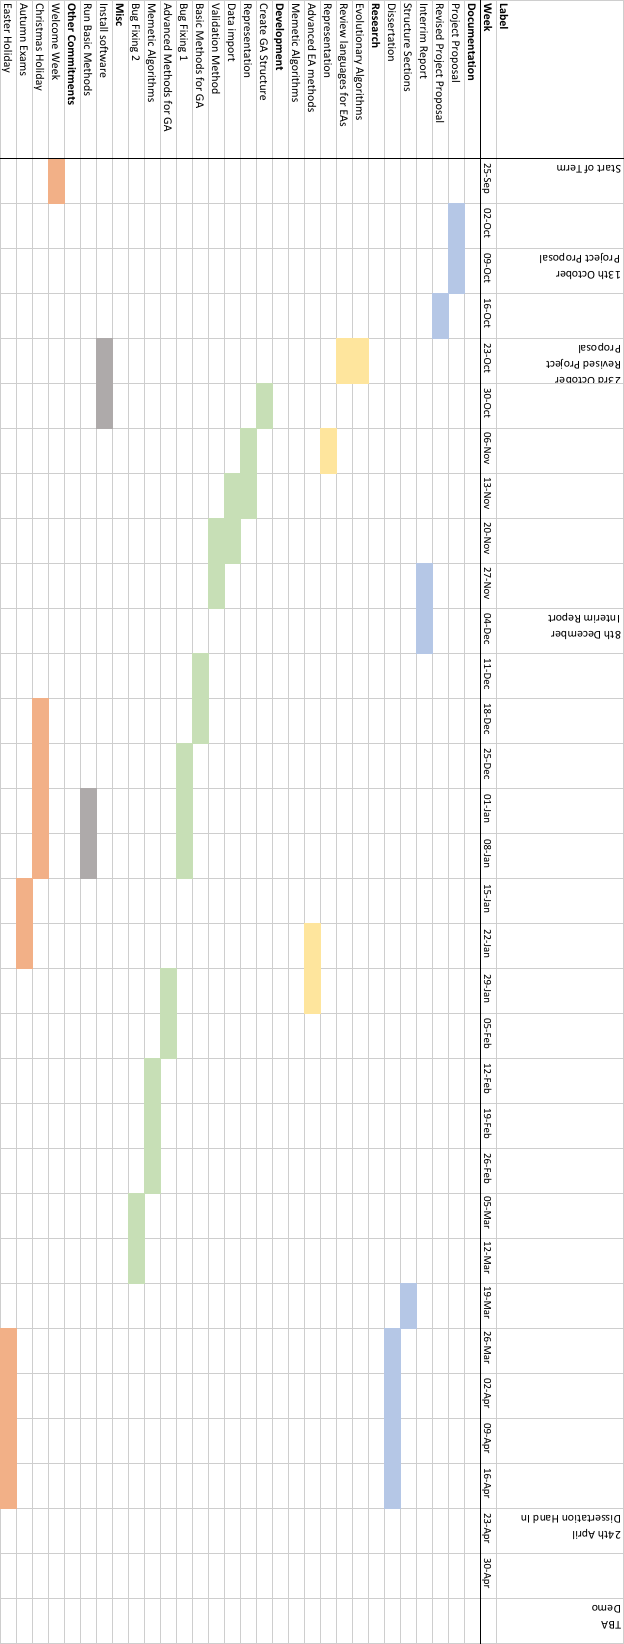
\includegraphics[width=17cm]{workPlan.png} %17cm is 21cm of A4 width - (2cm * 2) margins
\end{center}

\end{document}
